\chapter{Soluție propusă}
\section{Citire}

În acest subcapitol este prezentat modul de citire și stocare a metadatelor din manualul PDF. Procesul este împărțit în 3 etape: extragerea informațiilor de bază folosind PyMuPDF, asocierea unei culori de fundal pentru fiecare segment de text, extragerea imaginilor. Procesul se desfășoară conform următoarei diagrame.
\begin{figure}[H]
	\centering
	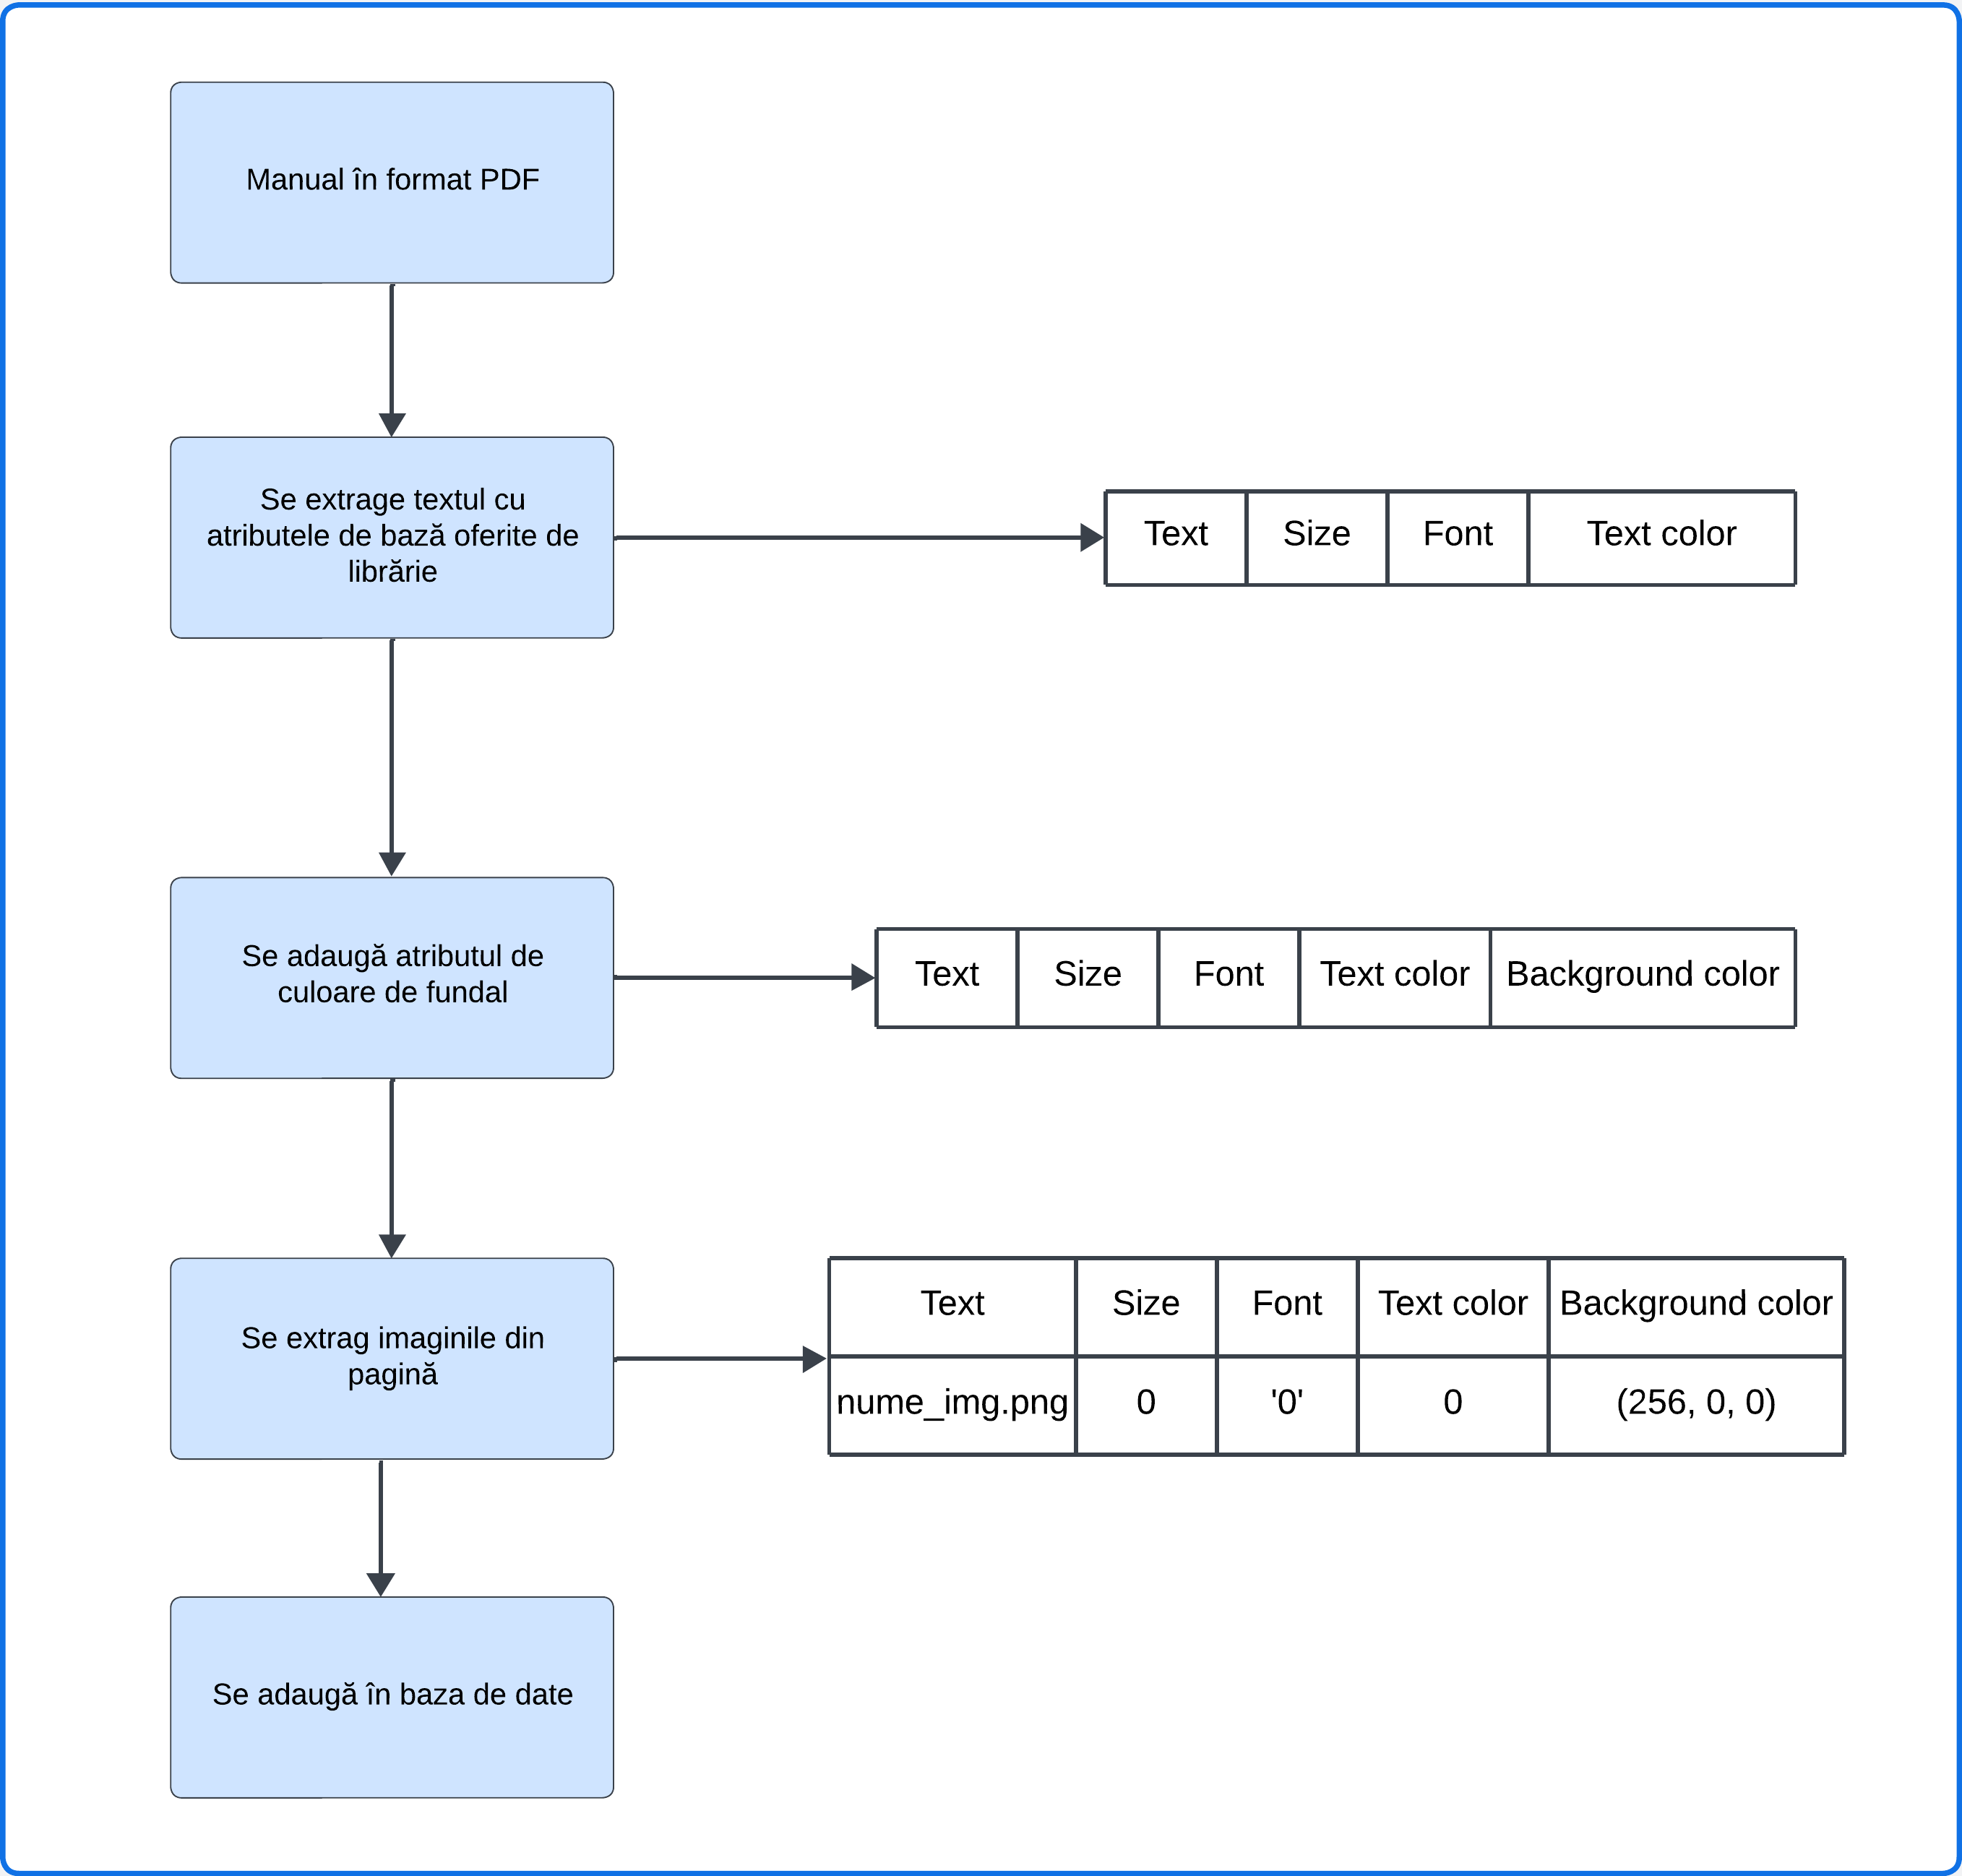
\includegraphics[scale=.5]{Figura4_1}
	\caption{Diagramă pentru subcapitolul de citire}
	\label{fig:Figura4_1}
\end{figure}

Pentru primul pas, se utilizează o funcție din librăria PyMuPDF care extrage majoritatea informațiilor importante despre documentul PDF. Această funcție extrage detalii precum culoarea textului, fontul, mărimea, coordonatele textului, dar și informații despre imagini cum ar fi tipul, lățimea, lungimea și transformările aplicate acestora.

Aceste informații sunt structurate ierarhic sub forma unor dicționare. Astfel, o pagină PDF conține un block, un block conține mai multe linii, iar o linie conține mai multe span-uri.
\begin{figure}[H]
	\centering
	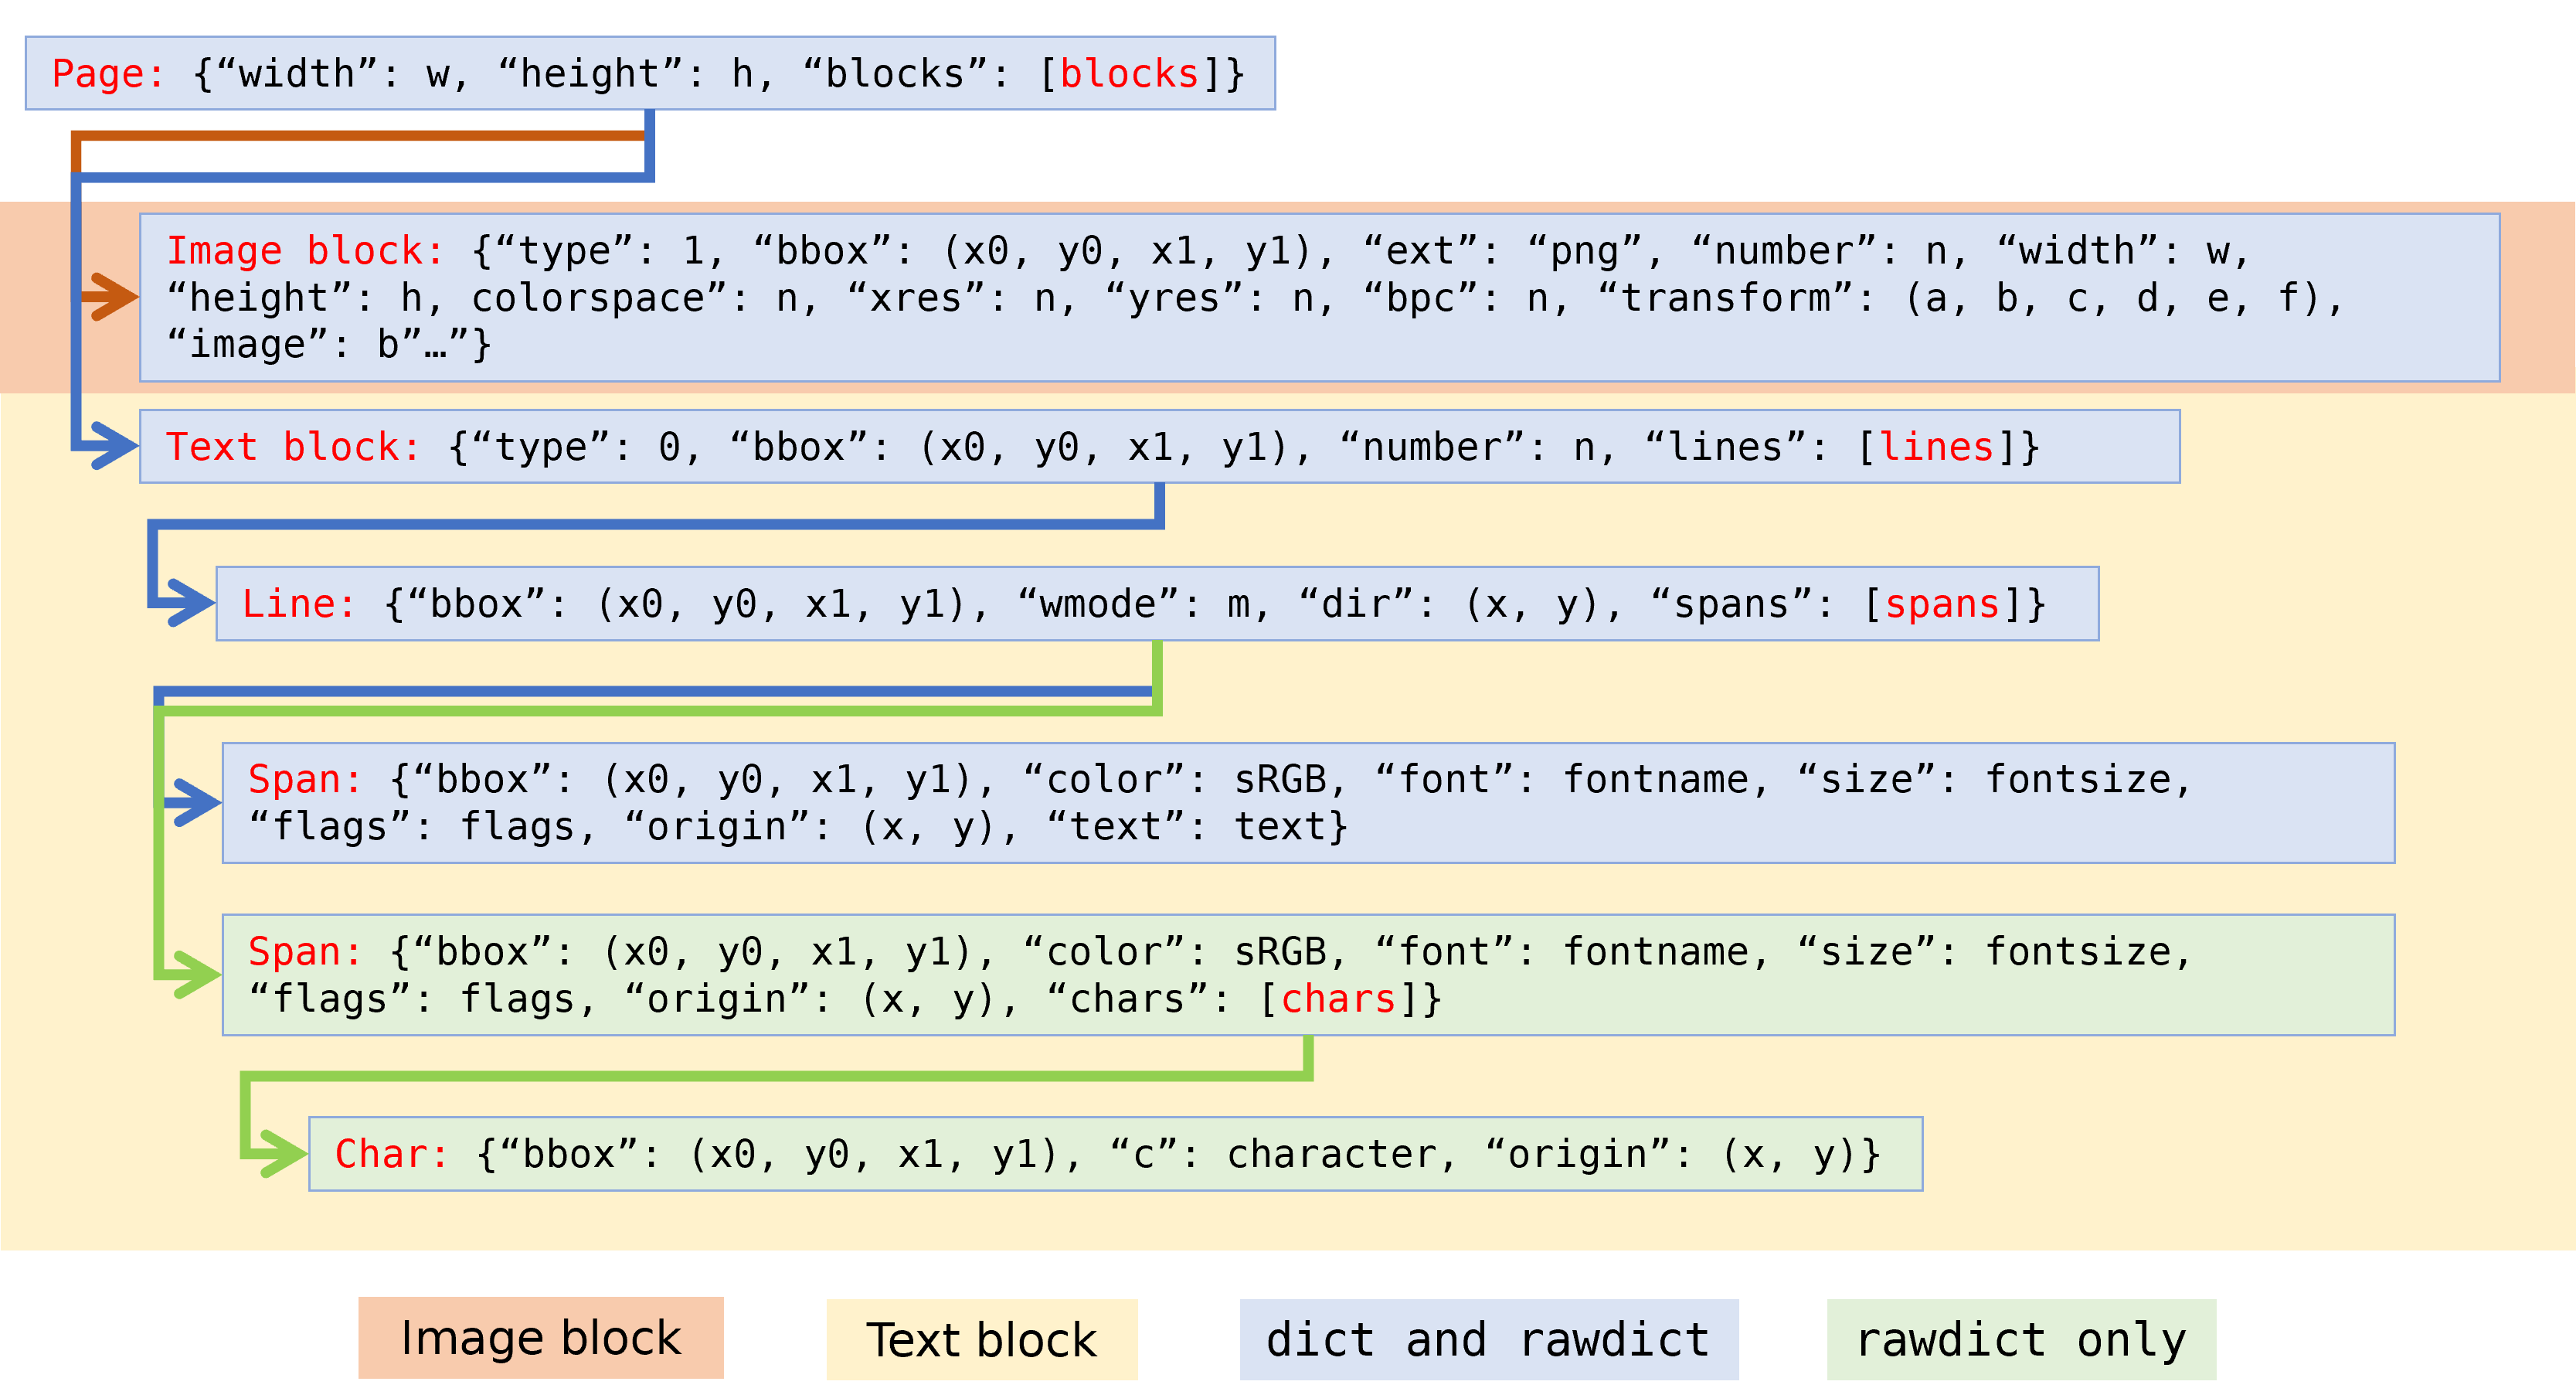
\includegraphics[scale=.15]{Figura4_2}
	\caption{Ierarhia informațiilor extrase din PDF}
	\label{fig:Figura4_2}
\end{figure}

Mărimea textului este măsurată în puncte (points), iar un punct reprezintă 1/72 inch. Pentru a extrage metadatele, se creează o funcție care va fi apelată la fiecare pagină. Aceasta va parcurge ierarhia pentru a obține informațiile necesare și pentru a le adăuga într-o listă de forma:
\begin{center}
	[Text, Size, Font, Text color]
\end{center}

\begin{lstlisting} [language=Python]
	def extract_pdf(path, page_nr):
		# Open PDF and extract text as a dictionary
		pdf = pymupdf.open(path)
		page = pdf.load_page(page_nr + 1)
		text_attributes_list = []
		text_attributes_dict = page.get_text('dict')
		
		for block in text_attributes_dict['blocks']:
			if block['type'] == 0:  # if type == 0 => text block
				for line in block['lines']:
					for span in line['spans']:
						text_attributes_list.append([span['text'], span['size'], 
						span['font'], span['color']])
			
		pdf.close()
		return text_attributes_list
\end{lstlisting}


\subsection{Culoarea de fundal}

Pentru a scrie textul în fișierul HTML final, este nevoie ca acesta să fie grupat în funcție de fragmentul din care face parte. Pentru unele porțiuni de text, singura metodă consistentă de grupare este cea bazată pe culoarea de fundal.

\vspace{3em}

În figura 4.3 este ilustrat un fragment de text cu fundal galben încadrat între două cerințe. Metodele de grupare implementate anterior nu au avut succes deoarece nu era clară delimitarea unui cu text cu fundal colorat de alte segmente de text. Astfel, a fost nevoie să se implementeze o metodă de determinare a culorii de fundal.
\begin{figure}[H]
	\centering
	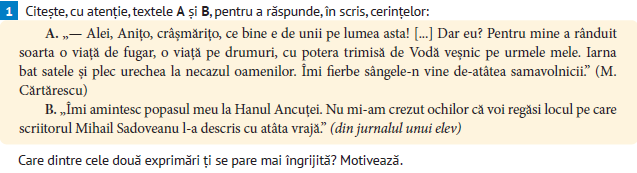
\includegraphics[scale=.8]{Figura4_3}
	\caption{Exemplu de text unde culoarea de fundal ajută la gruparea cuvintelor}
	\label{fig:Figura4_3}
\end{figure}

Pentru a extrage culoarea de fundal se va crea o funcție care verifică ce culoare apare predominant într-un block de text. Pașii urmați pentru a obține culoarea de fundal sunt:

\begin{itemize}
	\item transformarea paginii PDF într-un pixmap și ulterior într-o imagine;
	\item identificarea coordonatelor de la bounding box-urile fiecărei porțiune de text;
	\item determinarea celei mai frecvente culori din fiecare bounding box.
\end{itemize}

Pixmap-urile (pixel maps) sunt obiecte care stau la baza librăriei PyMuPDF. Ele reprezintă o suprafață cu un set de pixeli. Fiecare pixel este definit printr-un număr de bytes care reprezintă culoarea și transparența.

Bounding box-urile sunt chenare în care sunt încadrate block-urile de text. Acestea sunt prescurtate prin "bbox".

Înainte de a transforma pagina într-o imagine, este nevoie să o transformăm într-un pixmap. Acest lucru se face utilizând o funcție din librărie, căreia îi furnizăm o matrice de transformare. Această matrice modifică dimensiunile și înclinarea pixmap-urilor după cum urmează:
\begin{center}
	$\begin{bmatrix}
		a & b & 0\\
		c & d & 0\\
		e & f & 1
	\end{bmatrix}$
\end{center}

\noindent
Legendă coeficienți:
\begin{itemize}
	\item \(a\) - coeficient pentru a mări sau micșora lățimea (dacă este introdusă o valoare negativă, atunci poza se va întoarce invers de la stânga la dreapta).
	\item \(b\) - coeficient pentru a înclina imaginile orizontal; punctele de coordonate $A(x, y)$ vor deveni $A(x, y-b \cdot x)$.
	\item \(c\) - coeficient pentru a înclina imaginile vertical; punctele de coordonate $A(x, y)$ vor deveni $A(x - c \cdot y, y)$.
	\item \(d\) - coeficient pentru a mări sau micșora înălțimea (dacă este introdusă o valoare negativă, atunci poza se va întoarce invers de sus în jos).
	\item \(e\) - coeficient pentru a translata imaginea la stânga sau la dreapta; punctele de coordonate $A(x, y)$ vor deveni $A(x + e, y)$.
	\item \(f\) - coeficient pentru a translata imaginea mai sus sau mai jos; punctele de coordonate $A(x, y)$ vor deveni $A(x, y-f)$.
\end{itemize}

Exemplu de imagini pentru $b$ și $c$  modificat:
\begin{figure}[H]
	\centering
	\begin{subfigure}[t]{.5\textwidth}
		\centering
		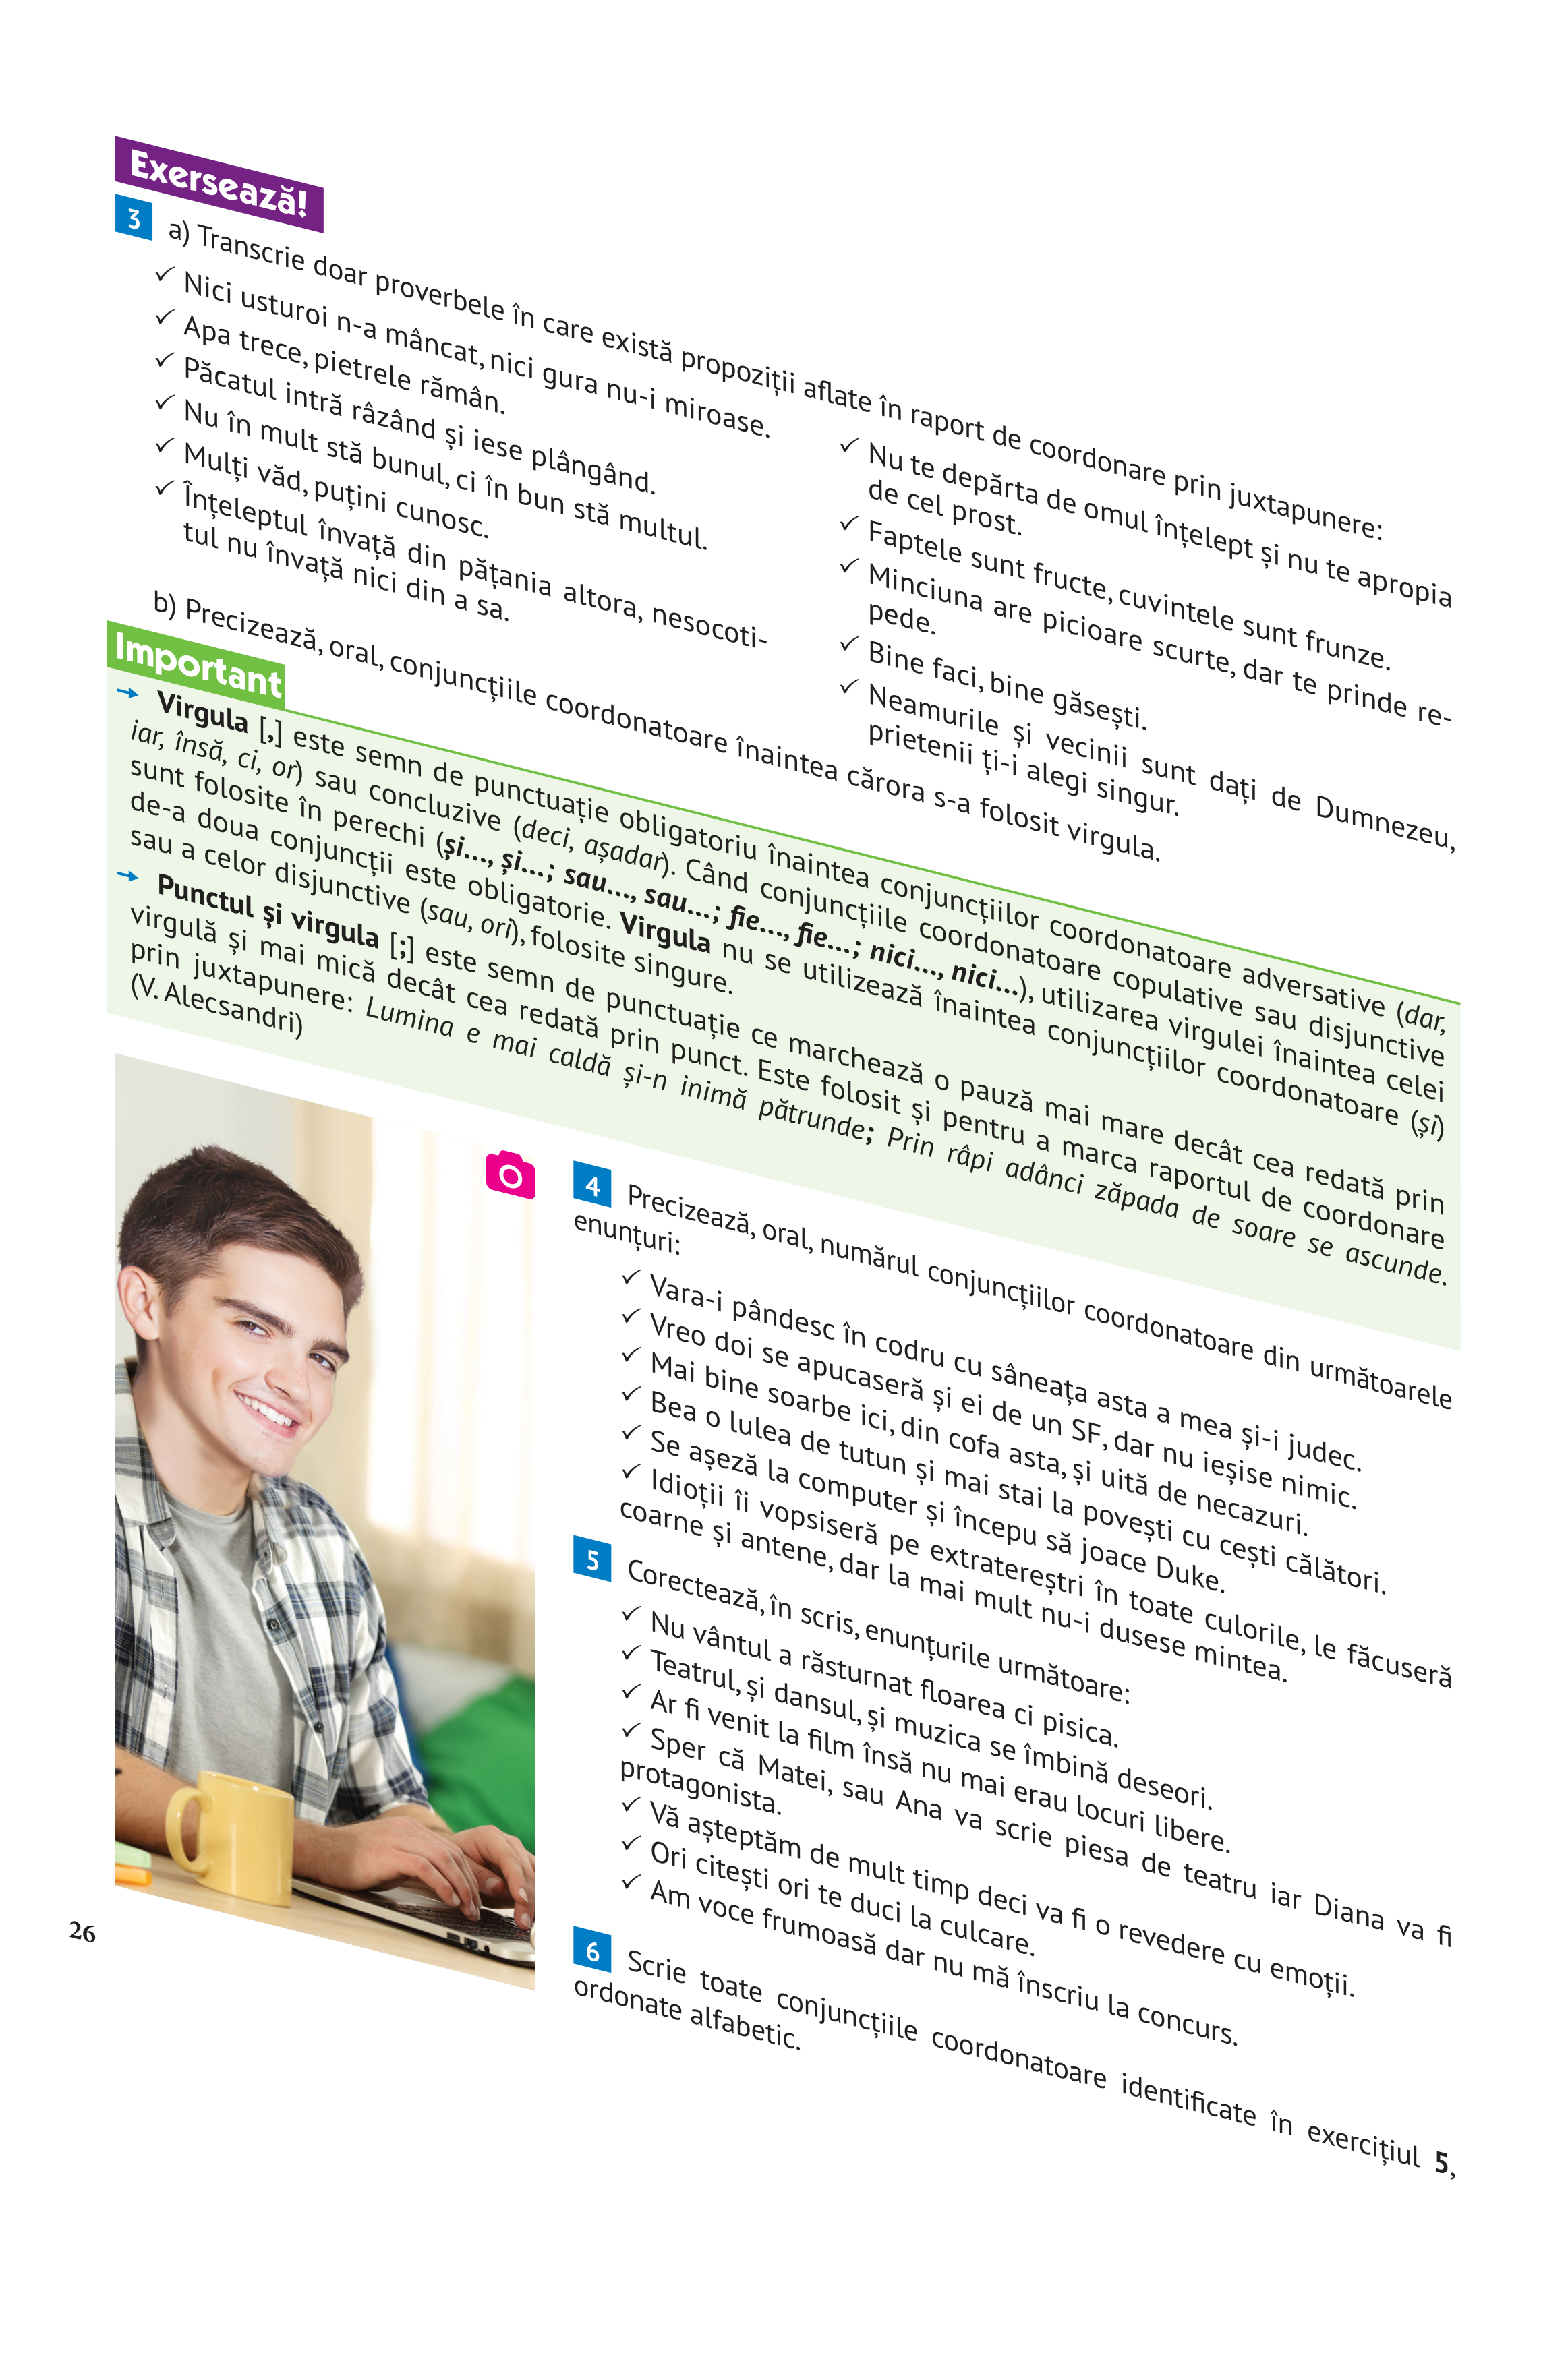
\includegraphics[width=.8\linewidth, height=.3\textheight]{Figura4_4a}
		\caption{Înclinare orizontală:
			$
			\begin{bmatrix}
				3 & 1 & 0\\
				0 & 3 & 0\\
				0 & 0 & 1
			\end{bmatrix}
			$}
		\label{fig:Figura4_4a}
	\end{subfigure}%
	\begin{subfigure}[t]{.5\textwidth}
		\centering
		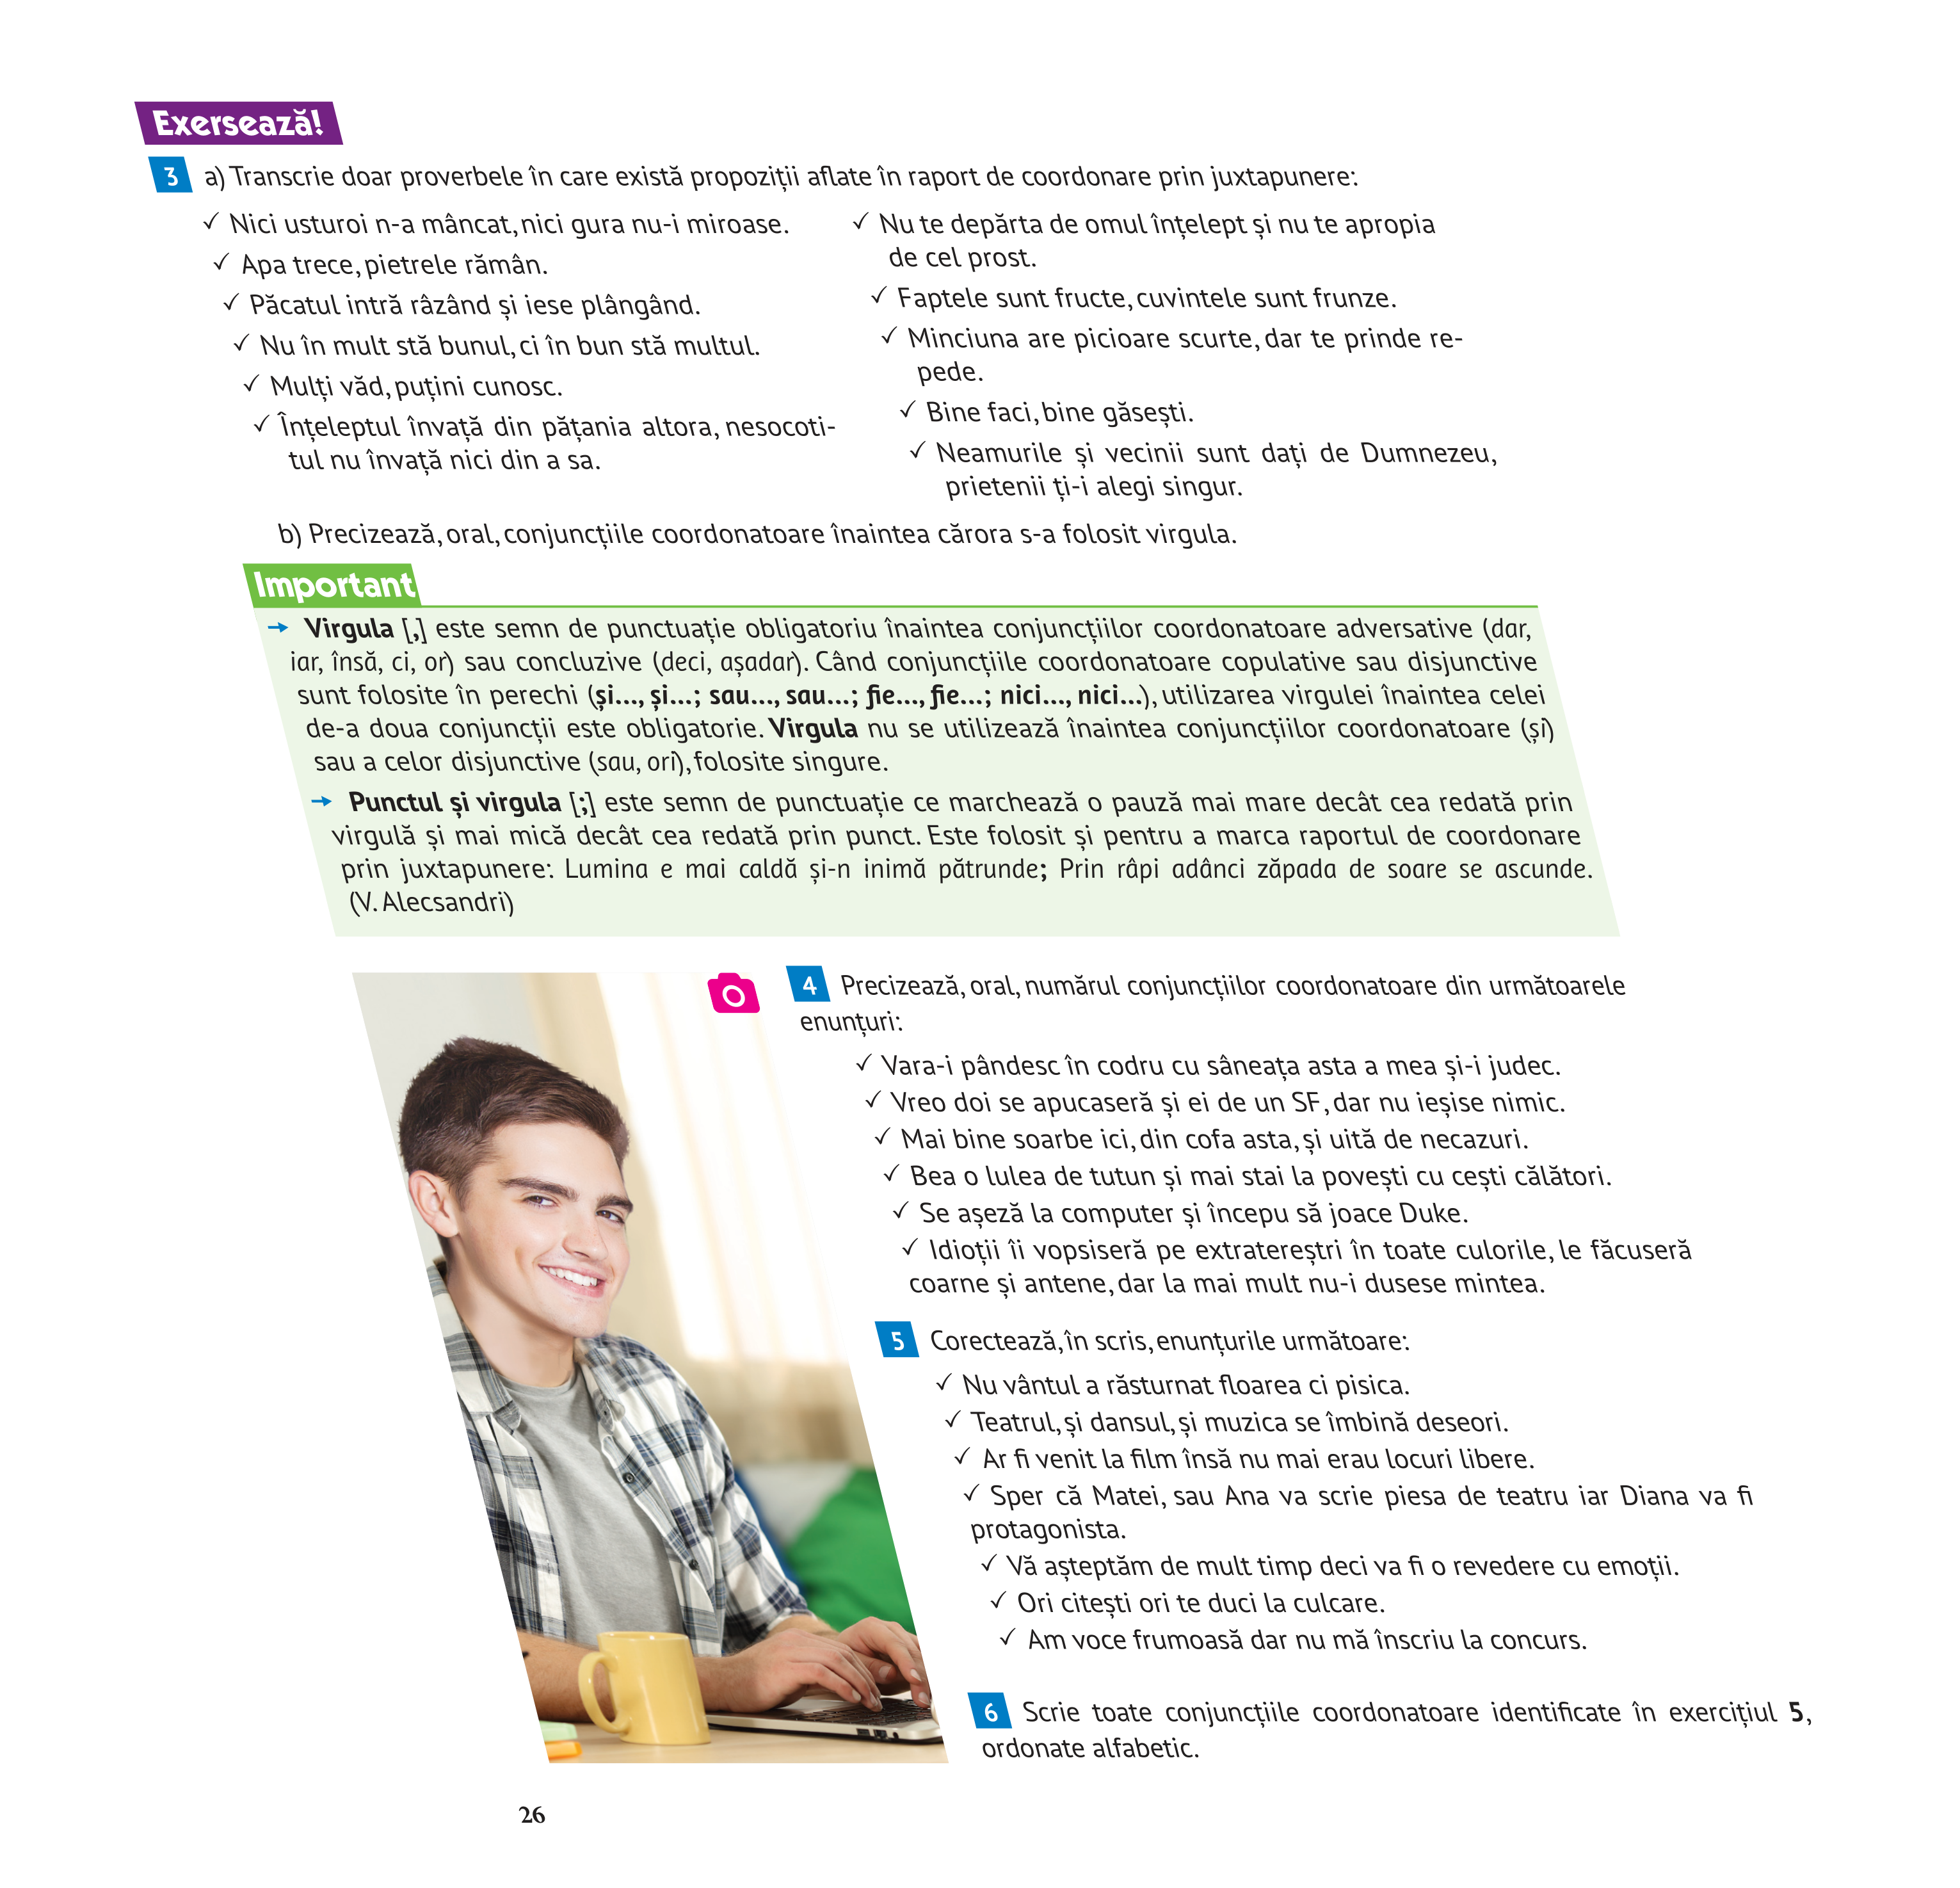
\includegraphics[width=.8\linewidth, height=.3\textheight]{Figura4_4b}
		\caption{Înclinare verticală:
			$
			\begin{bmatrix}
				3 & 0 & 0\\
				1 & 3 & 0\\
				0 & 0 & 1
			\end{bmatrix}
			$}
		\label{fig:Figura4_4b}
	\end{subfigure}
	\caption{Proprietăți ale matricii de transformare a imaginii}
	\label{fig:Figura4_4}
\end{figure}

Coeficienții care modifică rezoluția imaginii sunt $a$ și $d$. Aceștia sunt utilizați pentru a încadra textul cât mai precis posibil. Totuși, dacă se aleg valori prea mari, aplicația va rula mai lent din cauza rezoluției crescute.

\begin{figure}[H]
	\centering
	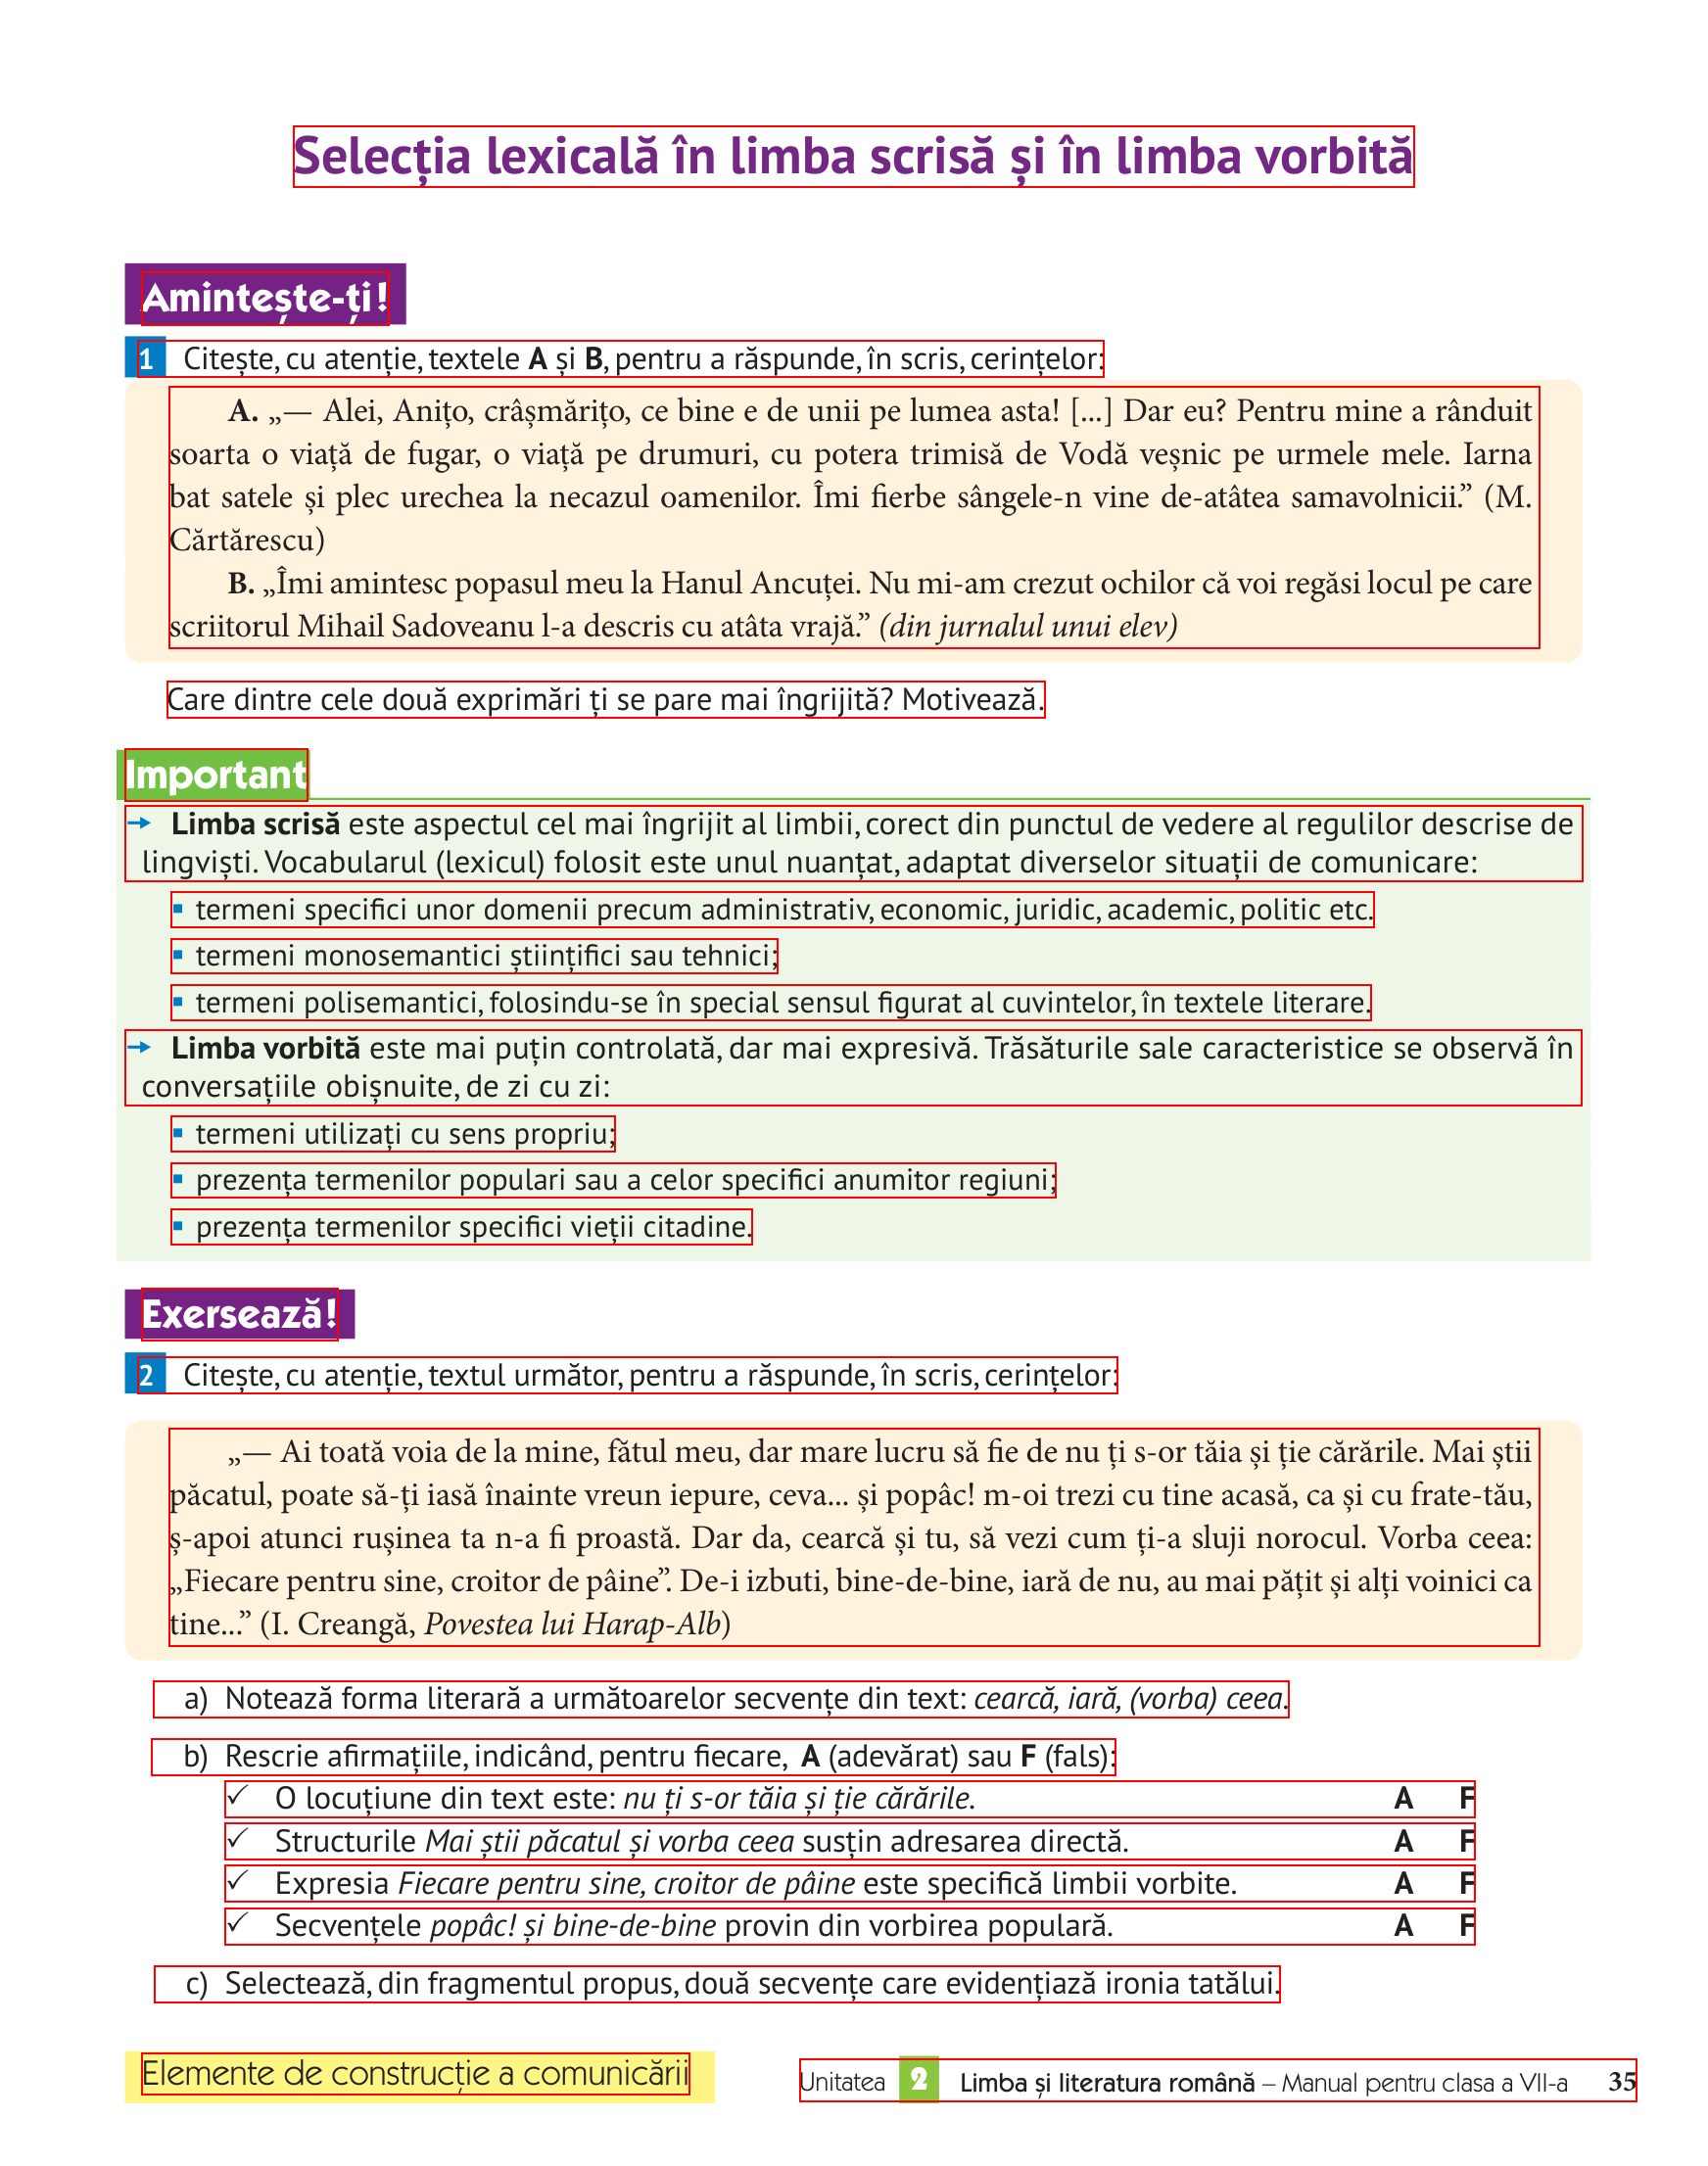
\includegraphics[scale=.2]{Figura4_5}
	\caption{Text încadrat în bbox-uri}
	\label{fig:Figura4_5}
\end{figure}

Pentru $a = d = 3$, fiecare imagine o să aibă dimensiunea de 2212x1744 px. Timpul mediu de rulare al programului pentru aceste dimensiuni ale imaginilor este de $0,4066$ secunde pe pagină. Pentru $a = d = 4$, fiecare imagine generată o să aibă dimensiunea de 2949x2325 px. Timpul mediu de rulare al programului pentru aceste dimensiuni ale imaginilor este de $0,5948$ secunde pe pagină.

După ce este găsită cea mai bună configurație pentru pagină, pixmap-ul se transformă într-o secvență de bytes, unde fiecare byte reprezintă toate informațiile necesare pentru a recrea o imagine. Câteva caracteristici sunt: identificarea tipului de imagine (PNG, JPG etc.), dimensiunea, culorile fiecărui pixel.

După acest pas, se extrage cea mai frecventă culoare din bbox. Pentru a face acest lucru, se analizează culoarea fiecărui pixel, iar cea mai des întâlnită culoare este returnată în format RGB.
\vspace{3em}
\begin{lstlisting} [language=Python]
	def extract_pdf(path, page_nr): 
		'''
		Open PDF and extract text as a dictionary
		'''
		
		# Turn page into a pixmap
		zoom_factor = 3
		matrix = pymupdf.Matrix(zoom_factor, zoom_factor)
		pixmap = page.get_pixmap(matrix=matrix)
		
		# Turn pixmap into an image
		image = Image.open(io.BytesIO(pixmap.tobytes()))
		img_border = pymupdf.Rect(0, 0, image.width, image.height)
		
		for block in text_attributes_dict['blocks']:
			if block['type'] == 0:  # if type is 0 then it is a text block
			bbox = block['bbox']
				x0, y0, x1, y1 = bbox
				x0_zoomed = x0 * zoom_factor
				y0_zoomed = y0 * zoom_factor
				x1_zoomed = x1 * zoom_factor
				y1_zoomed = y1 * zoom_factor
				rect = pymupdf.Rect(x0_zoomed, y0_zoomed, x1_zoomed, y1_zoomed)
				
				if img_border.contains(rect):  # Check if text block is in image
					color = pixmap.color_topusage(clip=rect)[1]  # Most used color
					block['bg_color'] = tuple(color)
		
		'''
		Append color to attributes list
		'''
		image.close()
		pdf.close()
		return text_attributes_list
\end{lstlisting}


\subsection{Extragerea imaginilor}

Extragerea imaginilor este un pas esențial în convertirea PDF-ului în HTML. În versiunea digitală este necesară apariția tuturor imaginilor prezente deja în cea de tipar. În cazul în care unele poze nu sunt citite, ele vor fi introduse manual ulterior.

Pentru a realiza această extragere, sunt parcurși următorii pași:
\begin{itemize}
	\item găsirea tuturor imaginilor din paginile PDF;
	\item verificarea formatului imaginii;
	\item verificarea imaginii dacă este inversată;
	\item salvarea imaginii într-un fișier.
\end{itemize}

Imaginile sunt returnate sub forma unei liste de elemente unde fiecare variabilă reprezintă o caracteristică a imaginii. Cu ajutorul referinței fiecărei imagini, aceasta se poate transforma într-un pixmap. Informațiile despre imagini sunt:
\begin{center}
	[xref, smask, width, height, bpc, colorspace, alt. colorspace, name, filter]
\end{center}

\begin{itemize}
	\item \textbf{xref}: referința de la imagine.
	\item \textbf{smask}: referința de la masca imaginii (masca imaginii este un nivel de transparență care se pune peste imagine).
	\item \textbf{width}: lățimea imaginii.
	\item \textbf{height}: înălțimea imaginii.
	\item \textbf{bpc}: numărul de biți (de obicei 8).
	\item \textbf{colorspace}: numele spațiului de culoare (RGB, CMYK, etc.).
	\item \textbf{alt. colorspace}: numele unui alt spațiu de culoarea (dacă este cazul).
	\item \textbf{name}: numele imaginii.
	\item \textbf{filter}: numele filtrului de decodare a imaginii (se referă la cum a fost comprimată imaginea în PDF).
\end{itemize}

CMYK este un spațiu de culoare și face referire la următoarele culori: cyan, magenta, yellow și key (black). Spațiul este predominant folosit pentru documentele care urmează a fi tipărite. La fel ca și CMYK, un alt spațiu de culoarea este RGB. Acronimul vine de la red, green, blue și este folosit pentru afișarea obiectelor pe orice tip de display.

O altă diferență între cele două spații de culoare este modul în care sunt folosite. Pentru a folosi formatul RGB se va alege un număr între 0 și 255 pentru fiecare culoarea. Fiecărui canal (R, G, B) i se atribuie 8 biți. Pentru formatul CMYK va fi ales un procent de la 0\% la 100\%.  
\begin{center}
	Albastru în format RGB:
	(0, 0, 255)
	
	Albastru în format CMYK:
	(100\%, 100\%, 0\%, 0\%)
\end{center}

La crearea manualului tipărit în Adobe InDesign, imaginile sunt ilustrate în format CMYK. Pentru a crea varianta digitală a unui manual, este necesar ca imaginile să fie transformate în format RGB, acesta fiind un spațiu nativ pentru display-uri \cite{anderson1996proposal}.

Pentru verificarea tipului de imagine este necesară verificarea numărului de componente ale unui pixel și nivelul de transparență. Dacă diferența dintre numărul de componente și nivelul de transparență este mai mare de 3, atunci imaginea este în format CMYK și trebuie să fie convertită în format RGB.

O variantă mai simplă ar fi fost să fie verificat atributul spațiului de culoare (colorspace). Această metodă nu ar fi funcționat deoarece pixmap-urile suportă doar trei spații de culoare: gray, RGB, CMYK. În general, există mai multe formatări de culoare. O metodă consistentă pentru verificare este cea descrisă mai sus în care este verificat numărul de componente al unui pixel.

În cazul unor imagini, există posibilitatea să fie inversate. Acest lucru se datorează modului în care au fost salvate pozele când au fost introduse în manual. Mai exact, a fost aplicată o matrice de transformare asupra lor. 

Pentru a verifica dacă imaginea este salvată în mod corect, se identifică matricea de transformare și, mai exact, primul parametru al acesteia. Dacă parametrul este negativ înseamnă că poza este inversată.

\vspace{3em}

Funcția care extrage imaginile este:
\vspace{1em}
\begin{lstlisting} [language=Python]
	def extract_pdf(path, page_nr):
		'''
		Open PDF and extract text as a dictionary
		'''
		
		'''
		Turn page into a pixmap
		'''
	
		# Extract images and save them to images directory
		image_list = page.get_images()
		for image_index, img in enumerate(image_list, start=1):
			xref = img[0]
			pix = pymupdf.Pixmap(pdf, xref)
			transform = page.get_image_info(xrefs=True)[image_index-1]['transform']
			if pix.n - pix.alpha > 3:
				pix = pymupdf.Pixmap(pymupdf.csRGB, pix)
			if transform[0] < 0:
				pix_image = Image.open(io.BytesIO(pix.tobytes()))
				pix_image = pix_image.transpose(method=Image.FLIP_LEFT_RIGHT)
				pix_image.save("manuale/Romana_nou/images/page_%s-image_%s.png" % (page_nr, image_index))
			elif img[5] != 'DeviceCMYK':
				pix.pil_save("manuale/Romana_nou/images/page_%s-image_%s.png" % (page_nr, image_index))
			else:
				pix.save("manuale/Romana_nou/images/page_%s-image_%s.png" % (page_nr, image_index))
			pix = None
		
		'''
		Turn page into a pixmap and append everything to the list
		'''
		
		image.close()
		pdf.close()
		return text_attributes_list
\end{lstlisting}
\vspace{1em}

Imaginile recunoscute de program și salvate au următorul format:

\begin{center}
	[numele pozei, 0 , '', 0, (256, 0, 0)]
\end{center}

Au fost alese aceste valori pentru a le diferenția de alte elemente de text, iar la culoarea de fundal a fost pus 256 pentru a fi clar că este o imagine. Un segment de text ar putea avea valori numai între 0 și 255.


\section{Curățare}

Al doilea pas este curățarea textului rezultat. Principalele elemente care vor fi eliminate sunt: spațiile goale, formulele de matematică și fizică, segmentele de text din subsolul paginii.

Formulele de matematică și fizică nu sunt recunoscute de librăria cu care este extras textul. Singurul lucru care este afișat la formule este \textbf{/uf072}. Având în vedere că toate formulele au același format, ele nu pot fi recunoscute, deci vor fi eliminate din baza de date.

Recunoașterea expresiilor matematice în documente digitale este o problemă care este studiată încă din anul 1967 \cite{anderson1967syntax} de Robert H. Anderson. În lucrările recente \cite{baker2010faithful}, au fost studiate metode de recunoaștere a formulelor prin OCR (Optical Character Recognition). Paginile PDF se transformă în imagini, iar expresiile sunt recunoscute după forma lor.

O alternativă care dă rezultate foarte bune este un algoritm  bazat pe mărimea obiectelor din PDF. Lucrarea \cite{wang2019extraction} de cercetare despre acest subiect a fost publicată în 2019 și prezintă un algoritm care are o precizie de 93,6 \%.

Pe lângă aceste formule, unele porțiuni de text vor fi scoase deoarece urmează să fie înlocuite cu imagini.

Pentru a realiza curățarea, se iterează prin lista de elemente și se verifică anumite criterii:
\begin{itemize}
	\item \textbf{Spații}:
	\begin{lstlisting} [language=Python]
		elif text == ' ':
		# Remove empty spaces
		i += 1\end{lstlisting}
	
	\item \textbf{Formule}:
	\begin{lstlisting} [language=Python]
		elif text == "\uf072":
		# Remove math/physics formulas
		i += 1\end{lstlisting}
	\item \textbf{Text înlocuit cu imagini}:
	\begin{lstlisting} [language=Python]
		elif bkgr_color == (255, 241, 214):
		# remove 'Citeste si' text box with specific background color (light beige)
		i += 1\end{lstlisting}
	\begin{figure}[H]
		\centering
		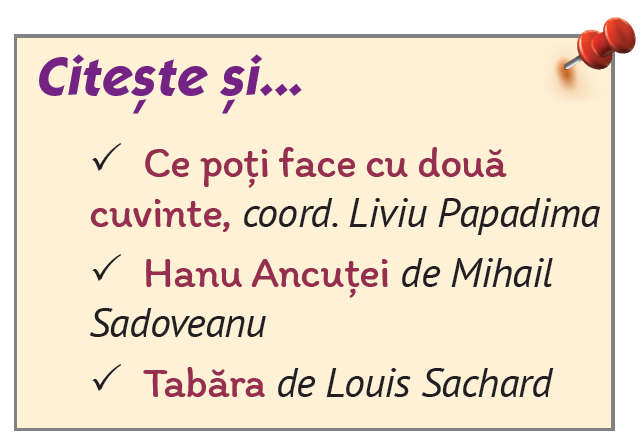
\includegraphics[scale=.3]{Figura4_6}
		\caption{Exemplu de text care va fi eliminat și înlocuit cu o imagine}
		\label{fig:Figura4_6}
	\end{figure}
	\vspace{8em}
	\item \textbf{Text din subsolul paginii}:
	\begin{lstlisting} [language=Python]
		elif size == 9.0 and font == 'ITCKabelStd-MediumRO' and text_attributes_list[i + 1][0] == ' – Manual pentru clasa a VII-a':
		# remove text besides page number
		i += 5\end{lstlisting}
	\begin{figure}[H]
		\centering
		
\includegraphics[scale=.8]{Figura4_7}
		\caption{Exemplu de text din subsolul paginii}
		\label{fig:Figura4_7}
	\end{figure}
\end{itemize}

Mai jos este o comparație între setul de date înainte și după ce a fost curățat.
\begin{table}[H]
	\centering
	\begin{minipage}{0.45\textwidth}
		\centering
		\begin{tabular}{|c|c|}
			\hline
			 & Text \\
			\hline
			1 & – Manual pentru clasa a VII-a \\
			\hline
			2 & Unitatea \\
			\hline
			3 & 19 \\
			\hline
			4 & 2 \\
			\hline
			5 & 4 \\
			\hline
			6 & Scrie câte un sinonim potrivit în \\
			\hline
			7 & text pentru fiecare dintre cuvintele: \\
			\hline
			8 &  \\
			\hline
			9 & 3 \\
			\hline
			10 & se înființă; \\
			\hline
			11 &  \\
			\hline
			12 & 3 \\
			\hline
			13 & să se-ntremeze; \\
			\hline
			14 &  \\
			\hline
			15 & 3 \\
			\hline
			16 & bat (satele); \\
			\hline
			17 &  \\
			\hline
			18 & 3 \\
			\hline
			19 & mă încolțește; \\
			\hline
		\end{tabular}
		\caption{Set de date înainte să fie curățat}
	\end{minipage}
	\hfill
	\begin{minipage}{0.45\textwidth}
		\centering
		\begin{tabular}{|c|c|}
			\hline
			& Text \\
			\hline
			1 & 4 \\
			\hline
			2 & Scrie câte un sinonim potrivit în \\
			\hline
			3 & text pentru fiecare dintre cuvintele: \\
			\hline
			4 & 3 \\
			\hline
			5 & se înființă; \\
			\hline
			6 & 3 \\
			\hline
			7 & să se-ntremeze; \\
			\hline
			8 & 3 \\
			\hline
			9 & bat (satele); \\
			\hline
			10 & 3 \\
			\hline
			11 & mă încolțește; \\
			\hline
		\end{tabular}
		\caption{Set de date după ce a fost curățat}
	\end{minipage}
\end{table}


\section{Grupare}

După ce a fost extras și curățat textul, acesta trebuie grupat. Gruparea se face pe mai multe niveluri. Primul nivel începe din interiorul textului de la cuvinte și ajunge până la fragmente întregi de text.

Două dintre cele mai des întâlnite motive pentru care segmentele de text se despart sunt: atunci când textul nu are același font peste tot, atunci când textul este scris pe un rând și se continuă pe altul.

\vspace{1em}
Pentru prima problemă va fi ilustrat un exemplu din manual în figura 4.8.
\begin{figure}[H]
	\centering
	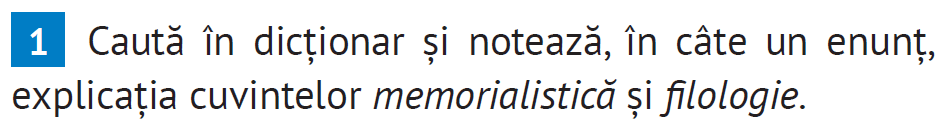
\includegraphics[scale=.35]{Figura5_1}
	\caption{Text preluat din manual}
	\label{fig:Figura5_1}
\end{figure}

Acest text se separă în felul următor:
\begin{table}[H]
	\centering
	\begin{tabular}{|l|l|l|}
		\hline
		Text                                               & Size & Font              \\ \hline
		"Caută în dicționar și notează, în câte un enunț," & 11   & "PT-Sans-Regular" \\ \hline
		"explicația cuvintelor"                            & 11   & "PT-Sans-Regular" \\ \hline
		"memorialistică"                                   & 11   & "PT-Sans-Italic"  \\ \hline
		"și"                                               & 11   & "PT-Sans-Regular" \\ \hline
		"filologie"                                        & 11   & "PT-Sans-Italic"  \\ \hline
	\end{tabular}
	\caption{Exemplu de text separat din cauza fontului și din cauza trecerii pe un rând nou}
\end{table}

Obiectivul de la acest pas este de a avea același font peste tot. Pentru a realiza acest lucru se vor transforma textele cu fonturi diferite (în cazul de față italic) într-un text cu font simplu, adăugându-i formatul HTML. Pentru a identifica ce texte se pot formata, se identifică numele fontului.
\begin{figure}[H]
	\centering
	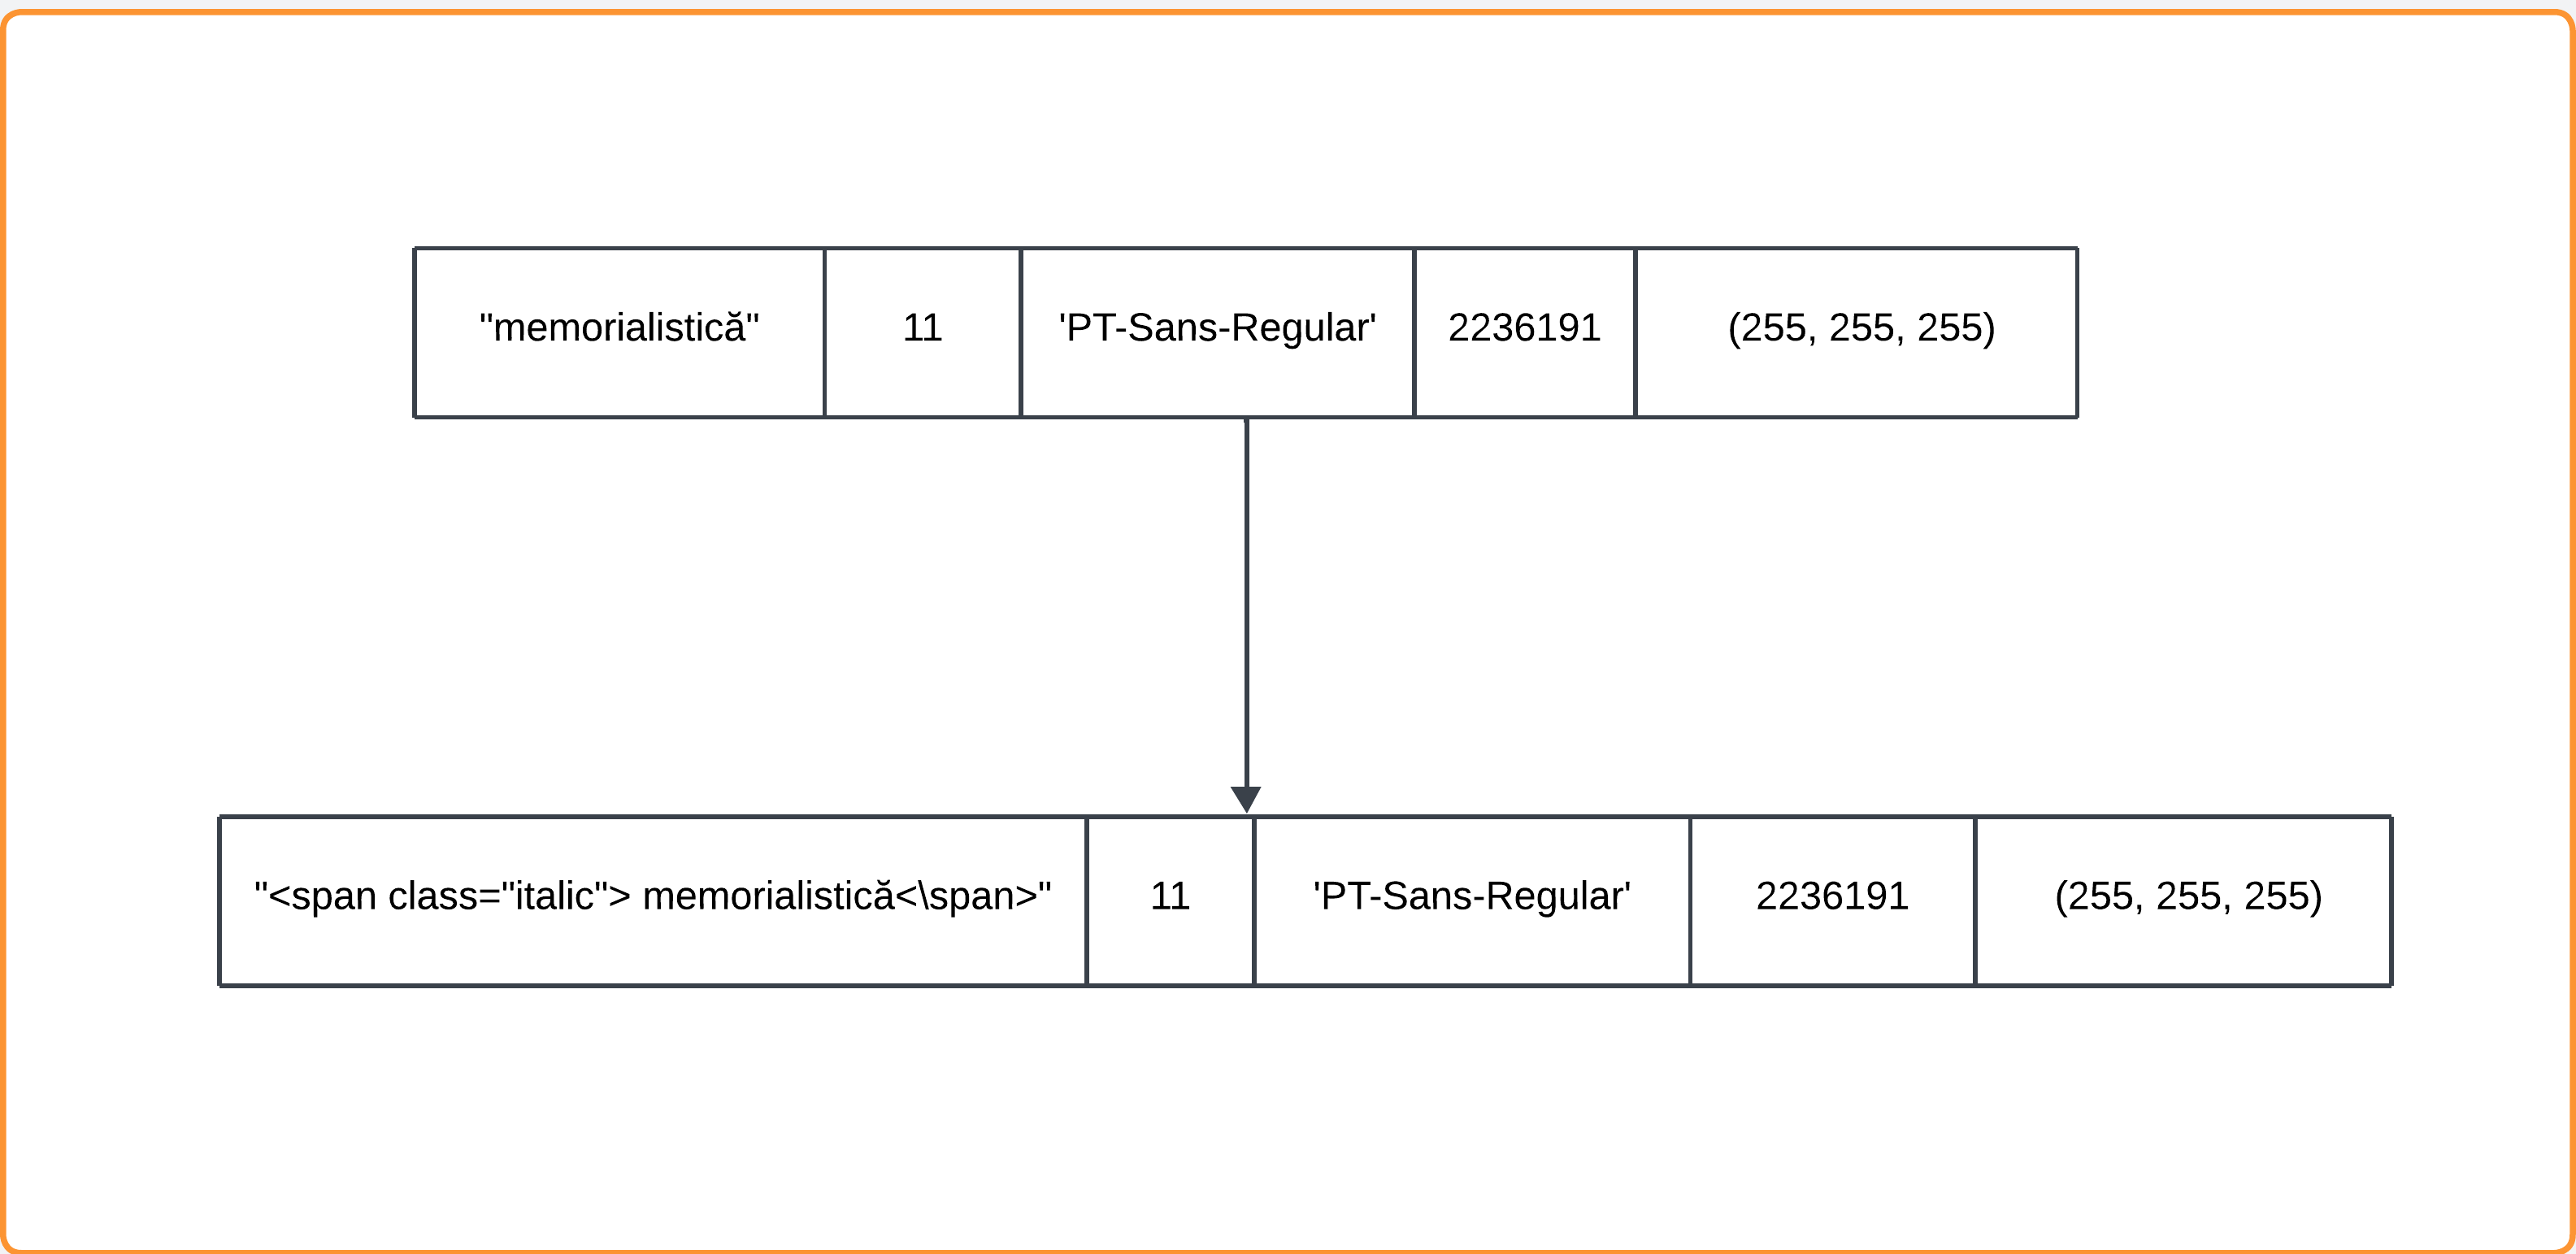
\includegraphics[scale=.45]{Figura5_2}
	\caption{Formatare a textului în HTML}
	\label{fig:Figura5_2}
\end{figure}

După ce este realizată schimbarea de font, se trece la următoarea problemă. Mai precis, cum se grupează textul scris pe mai multe rânduri.

Este construită o funcție în care se verifică pe rând dacă 2 elemente au aproximativ aceeași mărime (marjă de 0.2 points), același font și aceeași culoarea de fundal și după le combinăm.
\vspace{1em}
\begin{lstlisting} [language=Python]
	def combine_text(text_attributes_list):
		# Combine text with the same size, font and background color
		new_text_attributes_list = []
		previous_text = ""
		previous_size = 0
		previous_font = ""
		previous_color = 0
		previous_bg_color = (0, 0, 0)
		for element in text_attributes_list:
			text, size, font, color, bg_color = element
			if previous_size - 0.2 <= size <= previous_size + 0.2 and font == previous_font and bg_color == previous_bg_color:
				previous_text += " " + text
			else:
				if previous_text:
					new_text_attributes_list.append([previous_text, previous_size, previous_font, previous_color, previous_bg_color])
				previous_text = text
				previous_size = size
				previous_font = font
				previous_color = color
				previous_bg_color = bg_color
		
		if previous_text:
			new_text_attributes_list.append([previous_text, previous_size, previous_font, previous_color, previous_bg_color])
		
		return new_text_attributes_list
\end{lstlisting}
\vspace{1em}


După ce este realizată gruparea la primul nivel, se va aborda gruparea fragmentelor mai lungi.


\subsection{Exerciții}

Fragmentul de exerciții este cel mai des întâlnit paragraf dintr-un manual școlar. În figura 4.10 este ilustrat un astfel de exemplu.
\begin{figure}[H]
	\centering
	
\includegraphics[scale=.4]{Figura5_3}
	\caption{Exemplu de exercițiu}
	\label{fig:Figura5_3}
\end{figure}

Textul este extras conform pașilor anteriori.
\begin{table}[H]
	\centering
	\begin{tabular}{|p{5cm}|l|l|l|l|}
		\hline
		Text                                                                   & Size   & Font              & Text color & Background color \\ \hline
		"3"                                                                    & 9.8995 & "PT-Sans-Bold"    & 16777215   & (255, 255, 255)  \\ \hline
		"Alcătuiește familia lexicală a cuvintelor țară, pădure, bun, a face." & 10.78  & "PT-Sans-Regular" & 2236191    & (255, 255, 255)  \\ \hline
	\end{tabular}
	\caption{Segment de text după pașii de curățare și grupare}
\end{table}

Dacă pașii de grupare de dinainte au avut succes, în baza de date o să rămână numărul exercițiului și cerința. Doar numerele de la exerciții au mărimea de 9.8995 points și culoarea de 16777215. Așadar, se vor identifica numerele de la exerciții după aceste 2 criterii, va fi selectat textul următor, și vor fi introduse într-un block de exercițiu.
\vspace{1em}
\begin{lstlisting} [language=html]
	<div class="block-container">
		<span class="number">{text}</span>
		<div class="block-number-content">
			<p>{text2}</p>
		</div>
	</div>
	<p class="clear"></p>\n
\end{lstlisting}
\vspace{1em}

Variabilele text attributes list[i] și [i+1] reprezintă numărul exercițiului, respectiv textul care urmează după el. După ce am sunt transformate cele 2 elemente separate într-un singur block de HTML, ele sunt intorduse înapoi în baza de date.


\subsection{Liste ordonate}

De multe ori cerințele de la enunțuri conțin și subpuncte. Acestea sunt tratate sub forma unor liste ordonate din HTML (ordered list).
\begin{figure}[H]
	\centering
	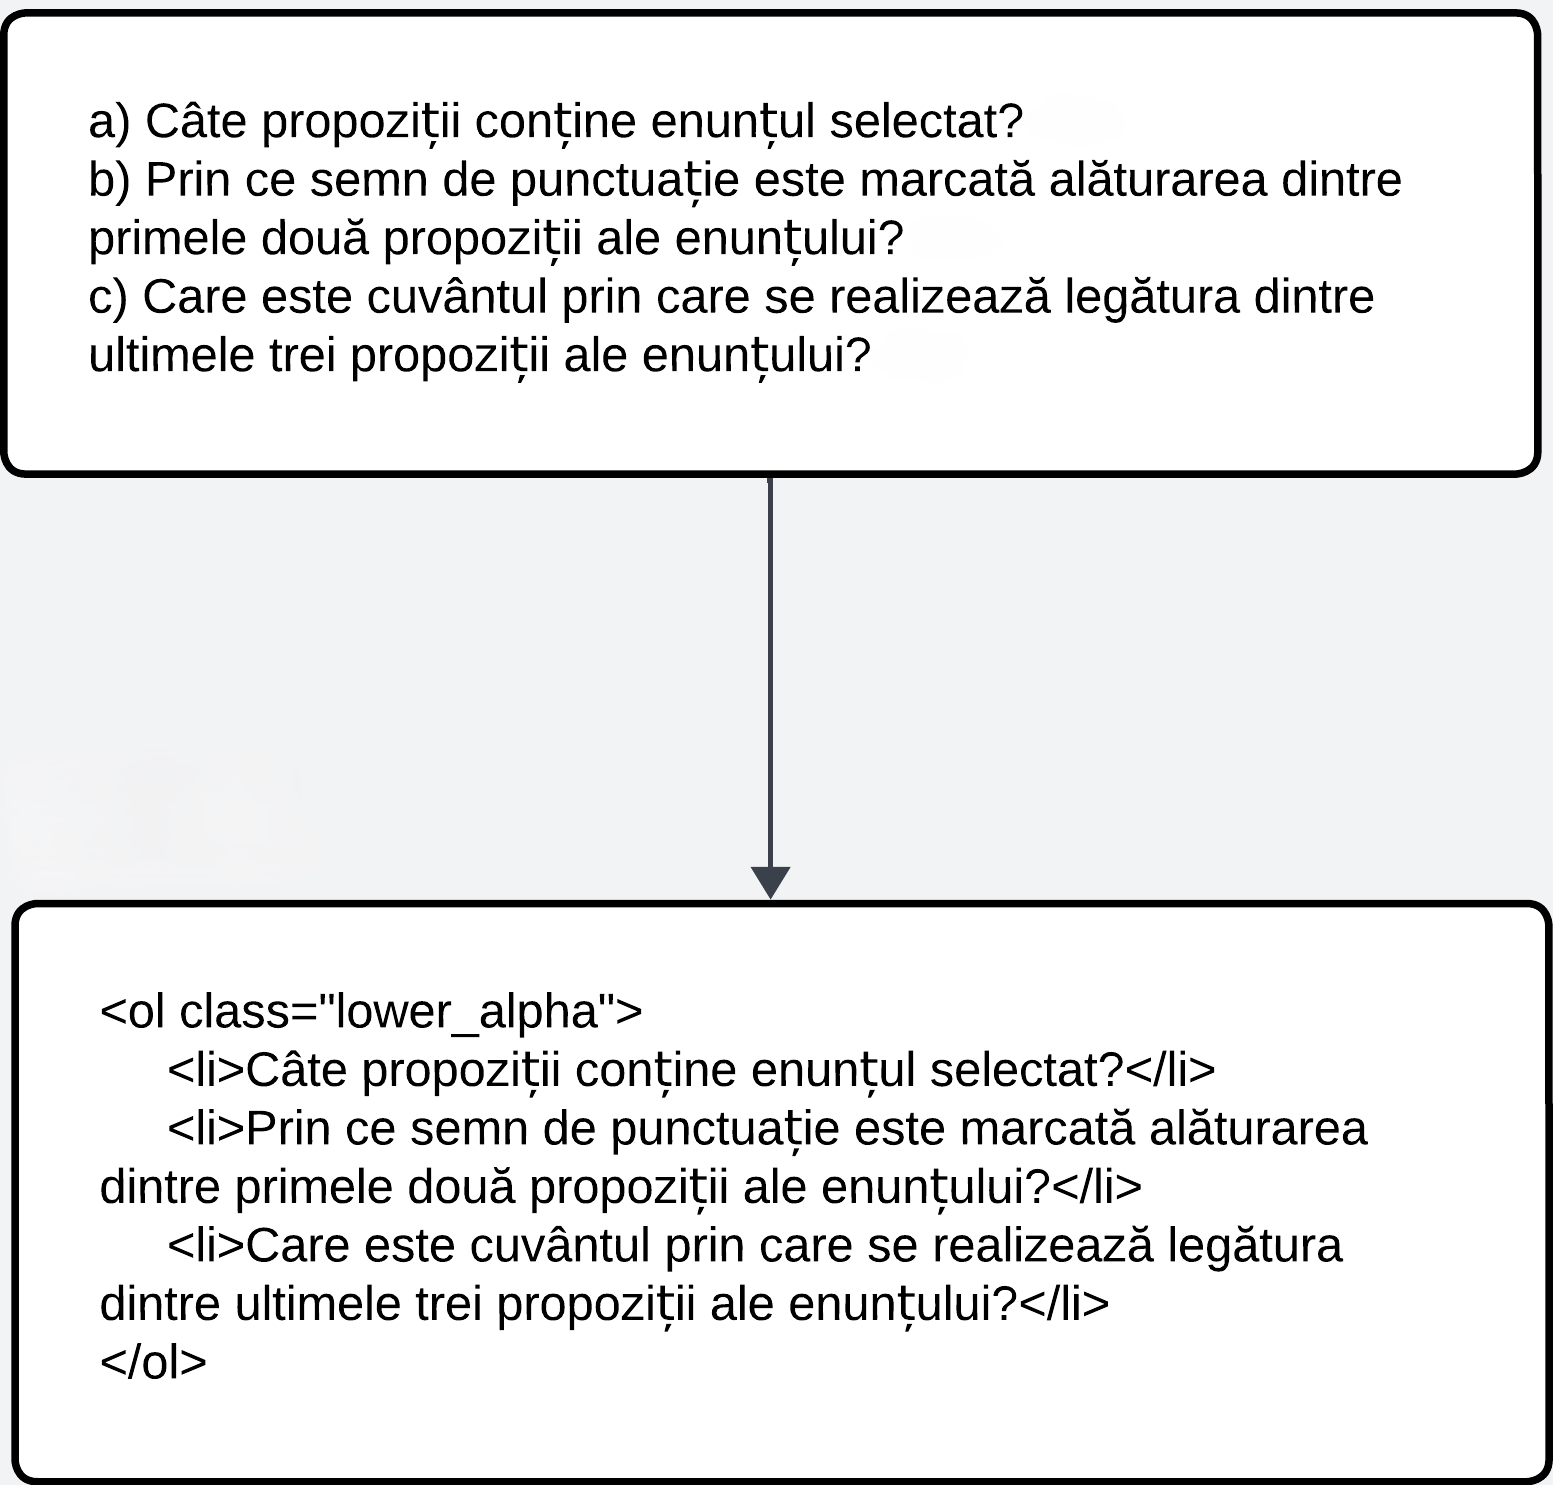
\includegraphics[scale=.5]{Figura5_4}
	\caption{Exemplu de liste transformate în HTML}
	\label{fig:Figura5_4}
\end{figure}

Atunci când este extras textul, aceste subpuncte sunt identificate ca o singură porțiune de text. Așadar, se desparte textul în funcție de numele subpunctului. 
\begin{center}
	pattern = r'\textbackslash s(?=[a-z]\textbackslash))
	
	result = re.split(pattern, text)
\end{center}

După aceea, se iterează prin lista de elemente cu subpuncte și se adaugă în formatul HTML.
\vspace{1em}
\begin{lstlisting} [language=Python]
	list_items_html = f'''
			<ol class="lower_alpha">
	'''
	for k in range(1, len(result)):
		list_items_html += f'''
				<li>{result[k][2:]}</li>
	'''
	list_items_html += f'''
			</ol>
	'''
\end{lstlisting}
\vspace{1em}

În baza de date, subpunctele sunt văzute ca o singură porțiune de text, iar ele vor fi separate și după reintorduse.


\subsection{Liste neordonate}

Listele neordonate care apar în manuale sunt de 3 feluri, în funcție de caracterul folosit pentru listare (bullet point etc.). Pentru fiecare caz va fi aplicat același algoritm.

Algoritmul propus este următorul: se creează 2 liste auxiliare; o listă mare în care vor fi toate elementele și o listă mică în care sunt doar elementele cu caracter special. În final, se va itera prin lista mare și va fi verificat dacă elementele au o structură de liste. După aceea, se va adăuga segmentul de text HTML care deschide și închide o listă neordonată (unordered list).


\subsection{Paragrafele "Important"}

Acest tip de paragrafe sunt motivul principal pentru care a trebuit să se extragă și culoarea de fundal a fiecărui segment de text. Aceste paragrafe au același format în care se începe cu numele "Important" care are un fundal verde închis, iar textul din cadrul acestui paragraf apare cu un verde mai deschis.
\begin{figure}[H]
	\centering
	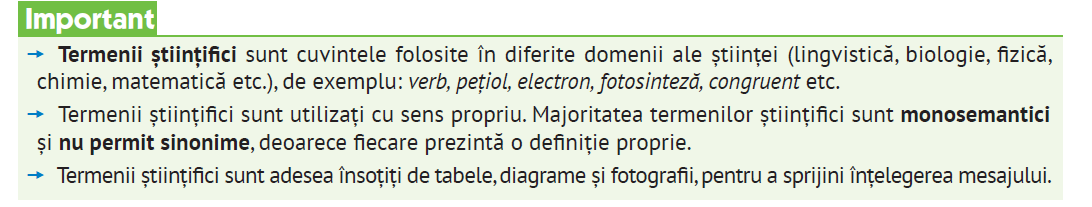
\includegraphics[scale=0.5]{Figura5_5}
	\caption{Exemplu de paragraf "Important"}
	\label{fig:Figura5_5}
\end{figure}

Problema de dinainte cu aceste tipuri de fragemente era faptul că nu se putea determina până unde se continuă un text cu fundal verde. Astfel, a fost nevoie de un nou atribut, și anume culoarea de fundal. Folosind această caracteristică, se poate verifica până unde se extinde textul dintr-un paragraf de tipul "Important".

Soluția găsită pentru acest tip de fragmente este următoarea: se grupează textul la fel ca la pașii anteriori, dacă există elemente care nu au fost grupate atunci ele vor fi adăugate conform culorii de fundal, se adaugă tot conținutul într-un div.

\vspace{1em}
\begin{lstlisting} [language=html]
	<h3 class="important">Important</h3>
	<div class="bkgr-imp">
		{text_imp}
	</div>
\end{lstlisting}

\section{Scriere}

După ce au fost parcurși toți pașii de curățare și grupare, mai rămâne doar partea de scriere. 

Se iterează prin lista de elemente și se verifică dacă acestea pot fi introduse în  fișierul HTML sau nu. Astfel, vor exista 3 tipuri de elemente în baza de date, conform tabelului de mai jos.
\begin{table}[H]
	\centering
	\begin{tabular}{|l|l|l|l|l|}
		\hline
		Text             & Size & Font        & Text color & Background color \\ \hline
		"some text"      & 0    & "0"         & 0          & (257, 0, 0)      \\ \hline
		"some image"     & 0    & "0"         & 0          & (256, 0, 0)      \\ \hline
		"other elements" & 123  & "some font" & 123        & (123, 123, 123)  \\ \hline
	\end{tabular}
	\caption{Tipuri de date rămase}
\end{table}

A fost realizată următoarea notație:

\begin{itemize}
	\item \textbf{Textul pregătit de scriere}: toate atributele vor fi notate cu 0, în afara de cel de la culoarea de fundal, care va fi notat cu 257. 
	\item \textbf{Imaginea}: toate atributele vor fi notate cu 0, în afara de cel de la culoarea de fundal, care va fi notat cu 256. 
	\item \textbf{Textul care nu este pregătit de scriere}: atributele nu se vor schimba. 
\end{itemize}

Au fost alese aceste caracteristici deoarece valorile culorii de fundal pot fi numai de la 0 la 255. Astfel, este mai ușor de identificat ce elemente sunt gata de introdus în fișierul HTML și ce elemente vor fi adăugate manual.